\documentclass{article}
\usepackage{fullpage}
\usepackage{parskip}
\usepackage{titlesec}
\usepackage{xcolor}
\usepackage[colorlinks = true,
            linkcolor = blue,
            urlcolor  = blue,
            citecolor = blue,
            anchorcolor = blue]{hyperref}
\usepackage[natbibapa]{apacite}
\usepackage{eso-pic}
\AddToShipoutPictureBG{\AtPageLowerLeft{\includegraphics[scale=0.7]{powered-by-Authorea-watermark.png}}}

\renewenvironment{abstract}
  {{\bfseries\noindent{\large\abstractname}\par\nobreak}}
  {}

\renewenvironment{quote}
  {\begin{tabular}{|p{13cm}}}
  {\end{tabular}}

\titlespacing{\section}{0pt}{*3}{*1}
\titlespacing{\subsection}{0pt}{*2}{*0.5}
\titlespacing{\subsubsection}{0pt}{*1.5}{0pt}

\usepackage{authblk}
\makeatletter
\renewcommand\AB@authnote[1]{\rlap{\textsuperscript{\normalfont#1}}}
\renewcommand\Authsep{,~\,}
\renewcommand\Authands{,~\,and }
\makeatother

\usepackage{graphicx}
\usepackage[space]{grffile}
\usepackage{latexsym}
\usepackage{textcomp}
\usepackage{longtable}
\usepackage{booktabs,array,multirow}
\usepackage{amsfonts,amsmath,amssymb}
\providecommand\citet{\cite}
\providecommand\citep{\cite}
\providecommand\citealt{\cite}
% You can conditionalize code for latexml or normal latex using this.
\newif\iflatexml\latexmlfalse
\DeclareGraphicsExtensions{.pdf,.PDF,.png,.PNG,.jpg,.JPG,.jpeg,.JPEG}

\usepackage[utf8]{inputenc}
\usepackage[T2A]{fontenc}
\usepackage[russian,greek,english]{babel}
\usepackage{CJKutf8}

\usepackage{multirow}
\usepackage[table,dvipsnames]{xcolor}
\usepackage{listings}
\usepackage{pifont}
\lstset{ %
  backgroundcolor=\color{white},   % choose the background color
  basicstyle=\footnotesize,        % size of fonts used for the code
  breaklines=true,                 % automatic line breaking only at whitespace
  captionpos=b,                    % sets the caption-position to bottom
  commentstyle=\color{OliveGreen},    % comment style
  keywordstyle=\color{BlueViolet},       % keyword style
  stringstyle=\color{black},     % string literal style
  language=[AlLaTeX]TeX,             % Set your language (you can change the language for each code-block optionally)
  frame=lrtb, %
  xleftmargin=\fboxsep, %
  xrightmargin=-\fboxsep, %
  moretexcs={not,like},
}

\def\onlyHTML#1{\iflatexml #1\fi}
\def\onlyPDF#1{\iflatexml\else #1\fi}

\newtheorem{theorem}{Theorem}
\newtheorem{proof}{Proof}
\newtheorem{lemma}{Lemma}


\begin{document}

\title{}


\author[ ]{michael}

\affil[ ]{}
\vspace{-1em}


\date{}

\begingroup
\let\center\flushleft
\let\endcenter\endflushleft
\maketitle
\endgroup

\begin{abstract}
A Showcase Article of all Authorea features in scholarly writing.

For discussion and history please consult \href{https://github.com/natejenkins/socialApp/issues/1601}{the GitHub issue}%
\end{abstract}%



\chapter{LaTeX Text}
\section{Text}
\subsection{Text in several Unicode locales}
\begin{tabular}{ll}
Bulgarian & \selectlanguage{russian}Български език\\
Greek & \selectlanguage{greek}Τα Ελληνικά υποστηρίζονται επαρκώς επίσης.\selectlanguage{english}\\
Chinese (Simplified) & \begin{CJK}{UTF8}{gbsn}简体中文\end{CJK}\selectlanguage{english},Yi Zi Ce Shi  \selectlanguage{english}\\
\end{tabular}

\subsection{Text styling}
\begin{itemize}
\item \textbf{bold},
\item \textit{italic},
\item \underline{underline},
\item {\color{red}c}o{\color{green}l}{\color{brown}o}{\color{blue}r}{\color{orange}s},
\item {\scriptsize sizes}, {\footnotesize sizes}, {\normalsize sizes}, {\large sizes}, {\Large sizes}, {\Huge sizes}
\item \verb|verbatim text|
\end{itemize}

\section{Inline}
\subsection{Citations}
\begin{itemize} 
\item cite: \cite{2016}, multiple: \cite{2016,Einstein_1922}
\item citet: \citet{2016}, multiple: \citet{2016,Einstein_1922},
\item citep: \citep{2016}, multiple: \citep{2016,Einstein_1922}, 
\item with page numbers \cite[pp.~2]{2016}, \cite[pp.~12-22]{Einstein_1922}
\end{itemize}

\subsection{Labels and references}\label{sec:labels}
Examples of references: 
\begin{itemize}
\item Subsection~\ref{sec:labels},
\item Figure~\ref{fig:example},
\item Equation~\ref{eq:lorenz}, and eq.~\ref{eq:coins}
\item Table~\ref{table:example}
\end{itemize}

\subsection{Block quotes}
\subsubsection{{\LaTeX} \{quote\}}
\begin{quote}
I do not like them in a box.
I do not like them with a fox.
I do not like them in a house.
I do not like them with a mouse.
I do not like them here or there.
I do not like them anywhere.
I do not like green eggs and ham.
I do not like them, Sam-I-am.
\end{quote}

\subsubsection{{\LaTeX} \{verbatim\}}
\begin{verbatim}
I do not like them in a box.
I do not like them with a fox.
I do not like them in a house.
I do not like them with a mouse.
I do not like them here or there.
I do not like them anywhere.
I do not like green eggs and ham.
I do not like them, Sam-I-am.
\end{verbatim}

\subsubsection{{\LaTeX} \{lstlisting\}}
\begin{lstlisting}
I do not like them in a box.
I do not like them with a fox.
I do not like them in a house.
I do not like them with a mouse.
I do not like them here or there.
I do not like them anywhere.
I do not like green eggs and ham.
I do not like them, Sam-I-am.
\end{lstlisting}

\subsection{Footnotes}
Example of a footnote\footnote{this one but also\footnote{a nested note}} and one more\footnote{that one}.

\subsection{Sub/superscripts}
In text we have textsuperscript\textsuperscript{sup} and textsubscript\textsubscript{sub}.

In math we have the hat $x^2$ and the underscore $x_2$.

\subsection{Math equations}
The Lorenz Equations (numbered, labeled as eq:lorenz and eq:coins):
\begin{eqnarray}\label{eq:lorenz}
\dot{x} & =\sigma(y-x)\nonumber  \\ 
\dot{y} & =\rho x-y-xz\nonumber  \\ 
\dot{z} & =-\beta z+xy\nonumber \\
\end{eqnarray}

The probability of getting \(k\) heads when flipping \(n\) coins is:
\begin{equation}\label{eq:coins}
P(E) = {n \choose k} p^k (1-p)^{ n-k}
\end{equation}


\subsubsection{Inline and display style}

We can say inline that for any $x \in \mathcal{N}$ we know that display style (unnumbered):
$$ x \geq 0 $$

\subsection{Code listings}
\begin{lstlisting}
\documentclass{article}
% document preamble
\begin{document}
% document body
Hello World!
\end{document}
\end{lstlisting}

\subsection{Links}
\begin{itemize}
\item A simple \verb|\url|: \url{https://www.authorea.com}
\item An abbreviated \verb|\href|: \href{https://www.authorea.com}{Authorea homepage}
\end{itemize}

\chapter{Chapter Structural}
\section{Section Structural}
\subsection{SubSection Structural}
\subsubsection{SubsubSection Structural}
\paragraph{Paragraph Structural}
All heading levels 

\section{Itemizations and enumerations (i.e. lists)}
\subsection{Enumerate}
\begin{enumerate}
\item enumerate one
\item enumerate two
\end{enumerate}

\subsection{Itemize}
\begin{itemize}
\item itemize one
\item itemize two
\end{itemize}

\subsection{Mixed and Nested}
\begin{enumerate}
\item mixed one
  \begin{itemize}
  \item nested item one
  \item nested item two
    \begin{enumerate}
    \item double nested one
    \item double nested two
    \end{enumerate}
  \item nested item three
  \end{itemize}
\item mixed two
  \begin{enumerate}
  \item nested enum one
  \item nested enum two
    \begin{itemize}
    \item double nested one
      \begin{enumerate}
      \item triple nested one
      \item triple nested two
      \end{enumerate}
    \item double nested two
    \end{itemize}
  \item nested enum three
    \begin{itemize}
    \item double nested item one
    \end{itemize}
  \end{enumerate}
\end{enumerate}

\section{AMSMath: proofs, theorems, lemmas}
\begin{theorem} Example theorem\end{theorem}
\begin{proof} Proof of example theorem \end{proof}
\begin{lemma} Follow-up example lemma \end[lemma]
\begin{theorem} Second example theorem \end{theorem}

\begin{figure}[h!]
\begin{center}
\includegraphics[width=0.70\columnwidth]{{{figures/1533513-10202702496355000-90486170-n/1533513-10202702496355000-90486170-n}}}
\caption{{\label{fig:example} Science cat approves of Showcase Article%
}}
\end{center}
\end{figure}

\section{Tables}
\colorlet{FreshGray}{gray!20!white}
\colorlet{FreshGreen}{green!20!white}
\colorlet{FreshYellow}{yellow!20!white}
\colorlet{FreshRed}{red!20!white}
\def\okcell{\cellcolor{FreshGreen}}
\def\avgcell{\cellcolor{FreshYellow}}
\def\badcell{\cellcolor{FreshRed}}
\def\nocell{\cellcolor{FreshGray}}

\begin{table}[h!]
\newcolumntype{g}{>{\columncolor{FreshGray}}c}
\begin{tabular}{ |g|c|c|c|c|  }
\hline
\multicolumn{5}{|c|}{Comparison of Sorting Algorithms} \\
\hline \rowcolor{FreshGreen} 
  \onlyHTML{\multirow{2}{*}{\okcell Name}}& \multicolumn{3}{|c|}{Performance} & \onlyHTML{\multirow{2}{*}{\okcell Memory}} \\ \cline{2-4}
  \onlyPDF{\multirow{-2}{*}{\okcell Name}} & Best & Average & Worst &  \onlyPDF{\multirow{-2}{*}{\okcell Memory}} \\
\hline
Quicksort & \okcell $n \log(n)$ & \okcell $n \log(n)$ & \badcell $n^2$ & \avgcell $\log n$ \\
Merge Sort & \okcell $n \log(n)$ & \okcell $n \log(n)$ & \okcell $n \log(n)$ & \badcell $n$ worst case\\
In-place merge Sort & \nocell -- & \nocell -- & \avgcell $n \log^2(n)$ & \okcell 1 \\
\hline
\end{tabular}
\caption{{\label{table:example} An advanced table}}}
\end{table}
Source for the tabular data: \url{http://en.wikipedia.org/wiki/Sorting\_algorithm}

\begin{figure}[h!]
\begin{center}
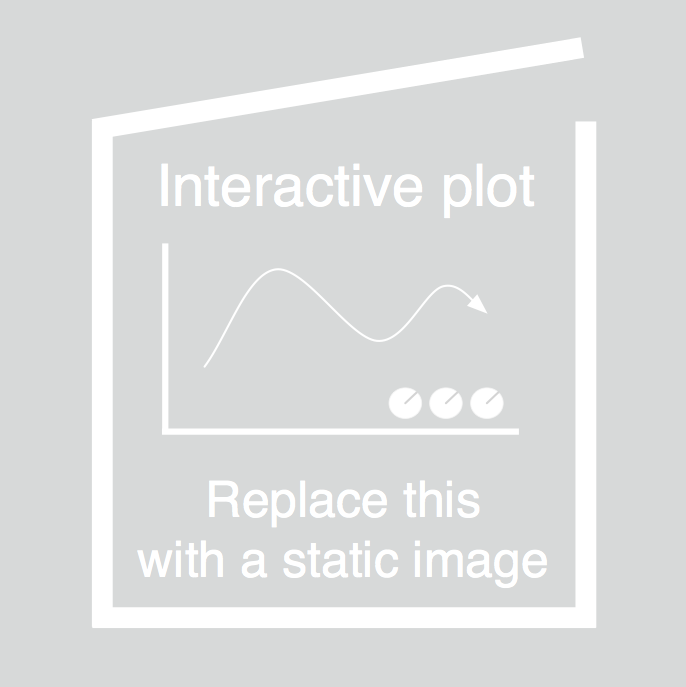
\includegraphics[width=0.70\columnwidth]{figures/interactive-figure-1470762309781/static.png}
\caption{An example interactive figure from our d3js
\href{https://www.authorea.com/templates/d3js}{template}%
}
\end{center}
\end{figure}

\chapter{Rich Text}

\section{Text~}

{\label{749446}}

\subsection{Text in several Unicode
locales~}

{\label{286674}}

\begin{longtable}[]{@{}ll@{}}
\toprule
Bulgarian & \selectlanguage{russian}Български език\tabularnewline
Greek & \selectlanguage{greek}Τα Ελληνικά υποστηρίζονται επαρκώς επίσης.\selectlanguage{english}\tabularnewline
Chinese (Simplified) & \begin{CJK}{UTF8}{gbsn}简体中文\end{CJK}\selectlanguage{english},Yi Zi Ce Shi \selectlanguage{english}\tabularnewline
\bottomrule
\end{longtable}

TODO: horizontal sizing? remove borders? tooltip in editor interferes
with insert?

\par\null

\subsection{Text styling~}

{\label{302732}}

\begin{itemize}
\tightlist
\item
  \textbf{bold}
\item
  \emph{italic}
\item
  underline
\item
  no colors :(
\item
  no sizes :(
\item
  no verbatim :(
\end{itemize}

\section{Inline~}

{\label{229592}}

\subsection{Citations~}

{\label{589961}}

\begin{itemize}
\tightlist
\item
  cite:~\cite{2016}, multiple:~\cite{2016,Einstein_1922}
\item
  citet:~\citealt{2016}, multiple:~\citealt{2016,Einstein_1922}
\item
  citep:~\citet{2016}, multiple:~\citet{2016,Einstein_1922}
\item
  with page numbers: no
\end{itemize}

\subsection{Labels and references~}

{\label{941883}}

Examples of references~

\begin{itemize}
\tightlist
\item
  Subsection:~{\ref{749446}}
\item
  Figure~{\ref{fig:example}}
\item
  Equation~{\ref{eq:coins}}
\item
  Table~{\ref{table:example}}
\end{itemize}

\subsection{Block quotes~}

{\label{815697}}

\begin{quote}
I do not like them in a box. I do not like them with a fox. I do not
like them in a house. I do not like them with a mouse. I do not like
them here or there. I do not like them anywhere. I do not like green
eggs and ham. I do not like them, Sam-I-am.
\end{quote}

No verbatim or listing.

\subsection{Footnotes~}

{\label{611925}}

No footnotes yet

\subsection{Sub/superscripts~}

{\label{872986}}

None yet

\subsection{Math equations~}

{\label{128245}}

MathQuill example:~\(P(E) = {n \choose k} p^k (1-p)^{ n-k}\)

Don't yet support display/reference-able math in richtext.

\subsection{Code listings~}

{\label{113134}}

None in richtext

\subsection{Links~}

{\label{406879}}

Simple URL: \href{http://www.authorea.com}{www.authorea.com}~and
abbreviated~\href{http://example.com}{example}.

\par\null

\chapter{RichText Chapter - none}

\section{RichText section/h1
structural}

{\label{757394}}

\subsection{RichText subsection/h2
structural}

{\label{978222}}

\subsubsection{RichText subsubsection/h3
structural}

{\label{129067}}

Richtext - no paragraph heading markup

All heading levels

\par\null

\section{Itemizations and Enumerations (i.e.
lists)}

{\label{835980}}

\subsection{Enumerate~}

{\label{517257}}

\begin{enumerate}
\tightlist
\item
  enumerate one
\item
  enumerate two
\end{enumerate}

\subsection{Itemize~}

{\label{479313}}

\begin{itemize}
\tightlist
\item
  itemize one
\item
  itemize two
\end{itemize}

\subsection{Mixed and nested~}

{\label{633244}}

TODO: Edge cases with switching between list levels (spurious items
created, spurious newlines on delete, ``saving\ldots{}'' bug when markup
mismatches, others)

TODO: I can't nest a numbered list here :( only an itemizeNested item
three

TODO: there is a blank space above i cant remove

TODO: Once saving\ldots{} is stuck on a nested list, the entire list
needs to be deleted for the block to succeed in sycning

\par\null

\begin{figure}[h!]
\begin{center}
\includegraphics[width=0.70\columnwidth]{{{figures/academics-are1/academics-are1}}}
\caption{Fun figure for showcase Beta richtext Insert
{\label{447587}}%
}
\end{center}
\end{figure}

\section{Tables~}

{\label{104557}}

No colors or advanced formatting yet.
See~{\ref{286674}} for a basic example.\selectlanguage{english}

\bibliographystyle{apacite}
\bibliography{bibliography/converted_to_latex.bib%
}

\end{document}

